\documentclass[11pt]{article}
\usepackage[margin=18mm,headheight=22pt]{geometry}
\usepackage{amsmath}
\usepackage{fontspec}
\usepackage{unicode-math}
\setmainfont{NewCM10}[Extension=.otf,UprightFont=*-Book,BoldFont=*-Bold,ItalicFont=*-BookItalic,BoldItalicFont=*-BoldItalic]
\setsansfont{NewCMSans10}[Extension=.otf,UprightFont=*-Book,BoldFont=*-Bold,ItalicFont=*-BookOblique,BoldItalicFont=*-BoldOblique]
\setmathfont{NewCMMath-Book.otf}
\usepackage{xcolor}
\definecolor{FAUblue}{HTML}{04316A}
\definecolor{Paperblue}{HTML}{EEF2F7}
\definecolor{EEIgold}{HTML}{CC9C42}
\usepackage{etoolbox,enumitem,booktabs,tabularx,array,needspace,microtype}
\usepackage[most]{tcolorbox}
\usepackage{titlesec,fancyhdr}
\usepackage[hidelinks]{hyperref}
\usepackage{draftwatermark}
\SetWatermarkText{Made by Thanate Amornjiraporn (Focus)}
\SetWatermarkColor{black!7}\SetWatermarkFontSize{30pt}\SetWatermarkAngle{45}
\setlength{\parindent}{0pt}
\setlength{\parskip}{5pt}
\setlist{itemsep=2pt,topsep=3pt,leftmargin=1.6em,beginpenalty=10000,endpenalty=10000}
\raggedbottom
\clubpenalty=10000 \widowpenalty=10000 \displaywidowpenalty=10000 \interlinepenalty=10000
\setcounter{secnumdepth}{0}
\setcounter{tocdepth}{1}
\pagestyle{fancy}\fancyhf{}
\fancyhead[L]{\small\sffamily\color{FAUblue} From Fundamentals to AI Apocalypse · EEI · Appendix B}
\fancyhead[R]{\small\sffamily Appendix B: Mathematical tools}
\fancyfoot[C]{\small\thepage}
\titleformat{\section}{\Large\bfseries\sffamily\color{FAUblue}}{}{0pt}{}
\titleformat{\subsection}{\large\bfseries\sffamily\color{FAUblue}}{}{0pt}{}
\titlespacing*{\section}{0pt}{16pt}{6pt}
\preto\section{\Needspace{8\baselineskip}}
\preto\subsection{\Needspace{6\baselineskip}}
\newtcolorbox{equationcard}[1]{colback=Paperblue,colframe=Paperblue,boxrule=0pt,arc=0pt,left=10pt,right=10pt,top=6pt,bottom=6pt,title={#1},fonttitle=\small\bfseries\sffamily,coltitle=FAUblue,before skip=8pt,after skip=8pt}
\newtcolorbox{workedbox}[1]{colback=white,colframe=EEIgold,boxrule=0pt,leftrule=3pt,arc=0pt,left=10pt,top=4pt,bottom=4pt,title={#1},fonttitle=\small\bfseries\sffamily,coltitle=FAUblue,attach title to upper={\par},before skip=8pt,after skip=8pt}
\newtcolorbox{recallbox}[1]{colback=white,colframe=FAUblue,boxrule=0pt,leftrule=3pt,arc=0pt,left=10pt,top=4pt,bottom=4pt,title={#1},fonttitle=\small\bfseries\sffamily,coltitle=FAUblue,attach title to upper={\par},before skip=8pt,after skip=8pt}
\usepackage{environ}
\newsavebox\measurebox
% Typeset the section once invisibly to measure it; start a new page if it will not fit in what is left.
\makeatletter
\newif\ifkeep@measuring
\NewEnviron{keepsection}{%
  \ifkeep@measuring \BODY \else
    \edef\keep@sec{\the\value{section}}\edef\keep@sub{\the\value{subsection}}%
    \setbox\measurebox\vbox{\hsize\linewidth\keep@measuringtrue\def\Needspace##1{}\BODY}%
    \setcounter{section}{\keep@sec}\setcounter{subsection}{\keep@sub}%
    \dimen2=\ht\measurebox \advance\dimen2\dp\measurebox
    \dimen@=\textheight
    \ifdim\pagegoal<\maxdimen
      \dimen@=\pagegoal \advance\dimen@-\pagetotal
      \ifdim\dimen2>\dimen@ \clearpage \dimen@=\textheight \fi
    \fi
    % if it fits, nothing inside may force an early break
    \ifdim\dimen2>\dimen@ \BODY \else \begingroup\def\Needspace##1{}\BODY\endgroup \fi
  \fi}
\makeatother
\newtcolorbox{notebox}{colback=Paperblue,colframe=Paperblue,boxrule=0pt,arc=0pt,left=8pt,right=8pt,top=4pt,bottom=4pt,before skip=6pt,after skip=6pt}
\newtcolorbox{plainbox}{colback=white,colframe=FAUblue,boxrule=0pt,leftrule=3pt,arc=0pt,left=10pt,right=8pt,top=4pt,bottom=4pt,before skip=6pt,after skip=8pt}
\usetikzlibrary{arrows.meta}
\title{\sffamily\bfseries\color{FAUblue}Appendix B: Mathematical tools}
\author{Electrical Engineering I \ensuremath{\cdot} Module 92315 \ensuremath{\cdot} Appendix B\\[2pt]\small From Fundamentals to AI Apocalypse · personal study guide}
\date{}
\begin{document}
\maketitle
\begingroup\footnotesize\setlength{\parskip}{0pt}\tableofcontents\endgroup
\clearpage

\Needspace{10\baselineskip}
{\large The mathematics the course assumes, in one place: line integrals and flux, vector arithmetic with the dot and cross products, the two-argument angle, linear systems from network analysis, and complex numbers in the j notation of AC analysis. Coordinate systems have their own page, Appendix A.}


\begin{keepsection}
\Needspace{15\baselineskip}
\section{B.1 Line integrals along a path}

\Needspace{12\baselineskip}
Many field quantities in the course are line integrals: the voltage between two points, the work done on a charge, the circulation of a field round a loop. A line integral adds up a quantity along a path \textit{C} from a start point \textit{P}\textsubscript{A} to an end point \textit{P}\textsubscript{B}. Cut the path into short pieces Δ\textit{s}\textsubscript{\textit{i}}, multiply each piece by the value of the quantity there, and let the pieces shrink to zero.

\begin{equationcard}{Line integral of a scalar}
\[ \begin{gathered} \int_{{P}_{\mathrm{A}}}^{{P}_{\mathrm{B}}} \, {f}({x},\, {y})\, \mathrm{d}{s}\, =\, \text{lim}\, \sum_{{i}=1}^{{n}} \, {f}({x}_{{i}},\, {y}_{{i}})\, Δ{s}_{{i}} \end{gathered} \]
{\small \emph{Read it as: “the integral of f along the path is the limit of the sum of f times each small piece of length”.}\par The limit is taken with \textit{n} \ensuremath{\to} \ensuremath{\infty} and every Δ\textit{s}\textsubscript{\textit{i}} \ensuremath{\to} 0; it exists when the result does not depend on how the path is cut.}
\end{equationcard}

\Needspace{11\baselineskip}
For a vector field such as \textit{E}, only the part of \textit{E} along the path counts, which the dot product picks out (B.4).

\begin{equationcard}{Line integral of a vector field}
\[ \begin{gathered} \int_{{P}_{\mathrm{A}}}^{{P}_{\mathrm{B}}} \, {E}\, \cdot \, \mathrm{d}{s}\, =\, \text{lim}\, \sum_{{i}=1}^{{n}} \, |{E}_{{i}}|\, |Δ{s}_{{i}}|\, \cos \, {α}_{{i}} \end{gathered} \]
{\small \emph{Read it as: “the integral of E dot d s: add the component of E along the path, times the path length”.}\par \textit{α}\textsubscript{\textit{i}} is the angle between the field and the path piece. A field perpendicular to the path contributes nothing; a field along the path contributes its full size. If the path is closed (\textit{P}\textsubscript{A} = \textit{P}\textsubscript{B}) the sign gets a ring: $\oint_{\mathrm{C}} $ \textit{E} \ensuremath{\cdot} d\textit{s}.}
\end{equationcard}

\Needspace{14\baselineskip}
\begin{center}
\begin{minipage}[t]{0.950\linewidth}\centering
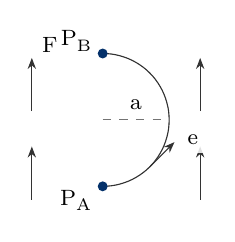
\begin{tikzpicture}[line join=round]
\draw[-{Stealth[length=4pt]},black!80] (0.769,-2.682) -- (0.769,-2.007);
\draw[-{Stealth[length=4pt]},black!80] (0.769,-1.557) -- (0.769,-0.882);
\draw[-{Stealth[length=4pt]},black!80] (2.907,-2.682) -- (2.907,-2.007);
\draw[-{Stealth[length=4pt]},black!80] (2.907,-1.557) -- (2.907,-0.882);
\filldraw[draw=black!80] (1.669,-2.513) -- (1.725,-2.511) -- (1.780,-2.506) -- (1.834,-2.497) -- (1.888,-2.484) -- (1.941,-2.468) -- (1.992,-2.449) -- (2.043,-2.426) -- (2.091,-2.400) -- (2.138,-2.371) -- (2.183,-2.339) -- (2.226,-2.304) -- (2.266,-2.266) -- (2.304,-2.226) -- (2.339,-2.183) -- (2.371,-2.138) -- (2.400,-2.091) -- (2.426,-2.043) -- (2.449,-1.992) -- (2.468,-1.941) -- (2.484,-1.888) -- (2.497,-1.834) -- (2.506,-1.780) -- (2.511,-1.725) -- (2.513,-1.669) -- (2.511,-1.614) -- (2.506,-1.559) -- (2.497,-1.505) -- (2.484,-1.451) -- (2.468,-1.398) -- (2.449,-1.347) -- (2.426,-1.296) -- (2.400,-1.248) -- (2.371,-1.201) -- (2.339,-1.156) -- (2.304,-1.113) -- (2.266,-1.073) -- (2.226,-1.035) -- (2.183,-1.000) -- (2.138,-0.968) -- (2.091,-0.939) -- (2.043,-0.913) -- (1.992,-0.890) -- (1.941,-0.871) -- (1.888,-0.855) -- (1.834,-0.842) -- (1.780,-0.833) -- (1.725,-0.828) -- (1.669,-0.826) -- (1.669,-0.826) -- (1.725,-0.828) -- (1.780,-0.833) -- (1.834,-0.842) -- (1.888,-0.855) -- (1.941,-0.871) -- (1.992,-0.890) -- (2.043,-0.913) -- (2.091,-0.939) -- (2.138,-0.968) -- (2.183,-1.000) -- (2.226,-1.035) -- (2.266,-1.073) -- (2.304,-1.113) -- (2.339,-1.156) -- (2.371,-1.201) -- (2.400,-1.248) -- (2.426,-1.296) -- (2.449,-1.347) -- (2.468,-1.398) -- (2.484,-1.451) -- (2.497,-1.505) -- (2.506,-1.559) -- (2.511,-1.614) -- (2.513,-1.669) -- (2.511,-1.725) -- (2.506,-1.780) -- (2.497,-1.834) -- (2.484,-1.888) -- (2.468,-1.941) -- (2.449,-1.992) -- (2.426,-2.043) -- (2.400,-2.091) -- (2.371,-2.138) -- (2.339,-2.183) -- (2.304,-2.226) -- (2.266,-2.266) -- (2.226,-2.304) -- (2.183,-2.339) -- (2.138,-2.371) -- (2.091,-2.400) -- (2.043,-2.426) -- (1.992,-2.449) -- (1.941,-2.468) -- (1.888,-2.484) -- (1.834,-2.497) -- (1.780,-2.506) -- (1.725,-2.511) -- (1.669,-2.513) -- cycle;
\fill[FAUblue] (1.669,-2.513) circle (0.063);
\fill[FAUblue] (1.669,-0.826) circle (0.063);
\node[anchor=east,fill=white,fill opacity=0.85,text opacity=1,inner sep=1pt,font=\footnotesize] at (1.579,-2.693) {P\textsubscript{A}};
\node[anchor=east,fill=white,fill opacity=0.85,text opacity=1,inner sep=1pt,font=\footnotesize] at (1.579,-0.664) {P\textsubscript{B}};
\draw[-{Stealth[length=4pt]},black!80] (2.266,-2.266) -- (2.581,-1.951);
\node[anchor=west,fill=white,fill opacity=0.85,text opacity=1,inner sep=1pt,font=\footnotesize] at (2.707,-1.951) {e\textsubscript{φ}};
\node[anchor=west,fill=white,fill opacity=0.85,text opacity=1,inner sep=1pt,font=\footnotesize] at (0.859,-0.720) {F};
\draw[black!55,dashed] (1.669,-1.669) -- (2.513,-1.669);
\node[fill=white,fill opacity=0.85,text opacity=1,inner sep=1pt,font=\footnotesize] at (2.091,-1.471) {a};
\end{tikzpicture}\par\smallskip{\small\raggedright \textbf{Work along a semicircle.} A constant force \textit{F} pushes along +\textit{y} while the path runs round the right half of a circle of radius \textit{a}, from \textit{P}\textsubscript{A} to \textit{P}\textsubscript{B}. At each point only the part of \textit{F} along \textit{e}\textsubscript{φ} does work.\par}\end{minipage}
\end{center}

\begin{workedbox}{Example \ensuremath{\cdot} work along a semicircle}
\Needspace{6\baselineskip}
\begin{enumerate}
\item Set up: path ρ = \textit{a}, \textit{φ} from \ensuremath{-}{\small\ensuremath{\dfrac{π}{2}}} to {\small\ensuremath{\dfrac{π}{2}}}, force \textit{F} = \textit{e}\textsubscript{y} \textit{F}\textsubscript{y}. On the circle the path element is d\textit{s} = \textit{e}\textsubscript{φ} \textit{a} d\textit{φ} (cylindrical coordinates, Appendix A).
\item The dot product \textit{e}\textsubscript{y} \ensuremath{\cdot} \textit{e}\textsubscript{φ} = cos \textit{φ} (from \textit{e}\textsubscript{φ} = \ensuremath{-}sin \textit{φ} \textit{e}\textsubscript{x} + cos \textit{φ} \textit{e}\textsubscript{y}), so \textit{F} \ensuremath{\cdot} d\textit{s} = \textit{a} \textit{F}\textsubscript{y} cos \textit{φ} d\textit{φ}.
\item Integrate: \textit{W} = \textit{a} \textit{F}\textsubscript{y} $\int_{-π/2}^{π/2} $ cos \textit{φ} d\textit{φ} = \textit{a} \textit{F}\textsubscript{y} [sin \textit{φ}] = 2\textit{a} \textit{F}\textsubscript{y}.
\end{enumerate}

Check: a constant force does the same work on every path between the same two points, so the straight route from \textit{P}\textsubscript{A} to \textit{P}\textsubscript{B}, of length 2\textit{a} along +\textit{y}, must give 2\textit{a} \textit{F}\textsubscript{y} too. It does.
\end{workedbox}
\end{keepsection}

\begin{keepsection}
\Needspace{17\baselineskip}
\section{B.2 Flux through a surface}

\Needspace{14\baselineskip}
Flux measures how much of a field passes through a surface. Picture a steady stream of particles crossing a flat frame: tilt the frame and fewer pass through, because the frame presents a smaller cross-section to the stream. The tilt enters through the angle between the flow and the frame's \textbf{surface normal}, the unit vector \textit{n} perpendicular to the frame that fixes which side counts as positive.

\begin{equationcard}{Flux through a flat surface in a uniform field}
\[ \begin{gathered} Ψ\, =\, {B}\, \cdot \, {A}\, =\, {B}\, {A}\, \cos \, {α} \\ {A}\, =\, {n}\, {A} \end{gathered} \]
{\small \emph{Read it as: “the flux is B dot A, the field times the area times the cosine of the tilt”.}\par \textit{A} is the oriented area: its size is the surface area and its direction the normal \textit{n}. \textit{α} is the angle between \textit{B} and \textit{n}, so a surface parallel to the field (\textit{α} = 90°) catches no flux.}
\end{equationcard}

\begin{equationcard}{Flux through any surface}
\[ \begin{gathered} Ψ\, =\, \int_{\mathrm{A}} \, {B}\, \cdot \, \mathrm{d}{A} \\ Ψ\, =\, \oiint_{\mathrm{A}} \, {B}\, \cdot \, \mathrm{d}{A} \end{gathered} \]
{\small \emph{Read it as: “the flux is the surface integral of B dot d A”.}\par Cut the surface into small flat pieces Δ\textit{A}\textsubscript{\textit{i}}, add \textit{B}\textsubscript{\textit{i}} \ensuremath{\cdot} Δ\textit{A}\textsubscript{\textit{i}} and let the pieces shrink. For a closed surface the normal points outwards by convention and the sign gets a ring. Two shortcuts: if \textit{B} is parallel to d\textit{A} everywhere, Ψ = $\int_{\mathrm{A}} $ \textit{B} d\textit{A}; if in addition \textit{B} is the same everywhere on the surface, Ψ = \textit{B} \textit{A}.}
\end{equationcard}

\begin{workedbox}{Example \ensuremath{\cdot} a tilted frame}
\Needspace{5\baselineskip}
\begin{enumerate}
\item A uniform field \textit{B} = 0.5 T crosses a flat frame of area \textit{A} = 0.02 m\textsuperscript{2} whose normal is tilted by \textit{α} = 60° from the field.
\item Ψ = \textit{B} \textit{A} cos \textit{α} = 0.5 T \ensuremath{\cdot} 0.02 m\textsuperscript{2} \ensuremath{\cdot} 0.5 = 0.005 Wb = 5 mWb.
\end{enumerate}

Check: at \textit{α} = 0 the frame faces the field squarely and catches the most, 10 mWb; at 90° it catches none. 1 Wb = 1 V s = 1 T m\textsuperscript{2}.
\end{workedbox}
\end{keepsection}

\begin{keepsection}
\Needspace{15\baselineskip}
\section{B.3 Vectors: components, length and direction}

\Needspace{12\baselineskip}
A \textbf{scalar} such as time \textit{t} or work \textit{W} is a number with a unit. A \textbf{vector} such as a force or a field also has a direction. Free vectors may be moved anywhere; bound vectors, such as a field value or a position vector, belong to one point. In Cartesian coordinates a vector is its three components along \textit{e}\textsubscript{x}, \textit{e}\textsubscript{y}, \textit{e}\textsubscript{z}.

\begin{equationcard}{Components}
\[ \begin{gathered} {a}\, =\, {a}_{\mathrm{x}}\, {e}_{\mathrm{x}}\, +\, {a}_{\mathrm{y}}\, {e}_{\mathrm{y}}\, +\, {a}_{\mathrm{z}}\, {e}_{\mathrm{z}}\, =\, ({a}_{\mathrm{x}},\, {a}_{\mathrm{y}},\, {a}_{\mathrm{z}})^{\mathrm{T}} \end{gathered} \]
{\small \emph{Read it as: “a is a x along e x plus a y along e y plus a z along e z”.}\par The notes write vectors as columns and use the transposed row (\ensuremath{\cdot})\textsuperscript{T} to save space. Two vectors are equal when all three components agree. The zero vector has length 0 and no direction.}
\end{equationcard}

\begin{equationcard}{Scaling, adding, subtracting}
\[ \begin{gathered} {c}\, {a}\, =\, ({c}\, {a}_{\mathrm{x}},\, {c}\, {a}_{\mathrm{y}},\, {c}\, {a}_{\mathrm{z}})^{\mathrm{T}} \\ {a}\, \pm \, {b}\, =\, ({a}_{\mathrm{x}}\, \pm \, {b}_{\mathrm{x}},\, {a}_{\mathrm{y}}\, \pm \, {b}_{\mathrm{y}},\, {a}_{\mathrm{z}}\, \pm \, {b}_{\mathrm{z}})^{\mathrm{T}} \end{gathered} \]
{\small Everything works component by component. Scaling by \textit{c} stretches the arrow by |\textit{c}| and reverses it for \textit{c} \ensuremath{<} 0; dividing by \textit{c} means scaling by {\small\ensuremath{\dfrac{1}{{c}}}}. Adding places the arrows head to tail (the parallelogram of forces).}
\end{equationcard}

\begin{equationcard}{Length and unit vector}
\[ \begin{gathered} |{a}|\, =\, \sqrt{{a}_{\mathrm{x}}^{2}\, +\, {a}_{\mathrm{y}}^{2}\, +\, {a}_{\mathrm{z}}^{2}} \\ {e}_{\mathrm{a}}\, =\, \dfrac{{a}}{|{a}|} \end{gathered} \]
{\small \emph{Read it as: “the unit vector along a is a divided by its length”.}\par Pythagoras in three dimensions. A unit vector has length 1 and only carries a direction; it exists for every \textit{a} \ensuremath{\neq} 0. Rules: |\ensuremath{-}\textit{a}| = |\textit{a}|, |\textit{c} \textit{a}| = |\textit{c}| |\textit{a}|, and the triangle inequality |\textit{a} + \textit{b}| \ensuremath{\leq} |\textit{a}| + |\textit{b}|.}
\end{equationcard}
\end{keepsection}

\begin{keepsection}
\Needspace{15\baselineskip}
\section{B.4 The dot product}

\Needspace{12\baselineskip}
The dot product turns two vectors into a number that says how much they point the same way. It is what picks out the component along a path in a line integral (B.1) and the component through a surface in a flux (B.2).

\begin{equationcard}{Dot product}
\[ \begin{gathered} {a}\, \cdot \, {b}\, =\, |{a}|\, |{b}|\, \cos \, {α} \\ {a}\, \cdot \, {b}\, =\, {a}_{\mathrm{x}}{b}_{\mathrm{x}}\, +\, {a}_{\mathrm{y}}{b}_{\mathrm{y}}\, +\, {a}_{\mathrm{z}}{b}_{\mathrm{z}} \end{gathered} \]
{\small \emph{Read it as: “a dot b is the length of a times the length of b times the cosine of the angle between them”.}\par \textit{α} is the angle between the arrows, 0 \ensuremath{\leq} \textit{α} \ensuremath{\leq} π. The component form follows because \textit{e}\textsubscript{x} \ensuremath{\cdot} \textit{e}\textsubscript{x} = 1 and \textit{e}\textsubscript{x} \ensuremath{\cdot} \textit{e}\textsubscript{y} = 0 for different unit vectors. The product is commutative and distributive, and \textit{a} \ensuremath{\cdot} \textit{a} = |\textit{a}|\textsuperscript{2}.}
\end{equationcard}

\begin{equationcard}{What it tells you}
\[ \begin{gathered} {α}\, =\, \arccos \, \dfrac{{a}\, \cdot \, {b}}{|{a}|\, |{b}|} \\ {b}_{\mathrm{a}}\, =\, \dfrac{{a}\, \cdot \, {b}}{|{a}|^{2}}\, {a} \end{gathered} \]
{\small Perpendicular: \textit{a} \ensuremath{\cdot} \textit{b} = 0. Parallel: \textit{a} \ensuremath{\cdot} \textit{b} = |\textit{a}| |\textit{b}|; antiparallel: \ensuremath{-}|\textit{a}| |\textit{b}|. The second line is the projection of \textit{b} onto the direction of \textit{a}. Cauchy–Schwarz: |\textit{a} \ensuremath{\cdot} \textit{b}| \ensuremath{\leq} |\textit{a}| |\textit{b}|.}
\end{equationcard}

\begin{workedbox}{Example \ensuremath{\cdot} angle and projection}
\Needspace{5\baselineskip}
\begin{enumerate}
\item \textit{a} = (1, 2, 2)\textsuperscript{T}, \textit{b} = (2, 0, 1)\textsuperscript{T}. Then \textit{a} \ensuremath{\cdot} \textit{b} = 2 + 0 + 2 = 4, |\textit{a}| = \ensuremath{\sqrt{1\, +\, 4\, +\, 4}} = 3 and |\textit{b}| = \ensuremath{\sqrt{5}}.
\item \textit{α} = arccos {\small\ensuremath{\dfrac{4}{3\sqrt{5}}}} \ensuremath{\approx} arccos 0.596 \ensuremath{\approx} 53.4°.
\item Projection of \textit{b} onto \textit{a}: {\small\ensuremath{\dfrac{4}{9}}} \textit{a} = ({\small\ensuremath{\dfrac{4}{9}}}, {\small\ensuremath{\dfrac{8}{9}}}, {\small\ensuremath{\dfrac{8}{9}}})\textsuperscript{T}.
\end{enumerate}

Check: the leftover \textit{b} \ensuremath{-} \textit{b}\textsubscript{a} = ({\small\ensuremath{\dfrac{14}{9}}}, \ensuremath{-}{\small\ensuremath{\dfrac{8}{9}}}, {\small\ensuremath{\dfrac{1}{9}}})\textsuperscript{T} has dot product {\small\ensuremath{\dfrac{14}{9}}} \ensuremath{-} {\small\ensuremath{\dfrac{16}{9}}} + {\small\ensuremath{\dfrac{2}{9}}} = 0 with \textit{a}, so it is perpendicular to \textit{a}, as a projection's remainder must be.
\end{workedbox}
\end{keepsection}

\begin{keepsection}
\Needspace{16\baselineskip}
\section{B.5 The cross product}

\Needspace{13\baselineskip}
The cross product turns two vectors into a third that stands perpendicular to both. Its length is the area of the parallelogram the two span, and its direction follows the right-hand rule: thumb along \textit{a}, index finger along \textit{b}, middle finger along \textit{a} \ensuremath{\times} \textit{b}. It appears wherever a force or a field turns at right angles, as in the magnetic force on a moving charge.

\begin{equationcard}{Cross product}
\[ \begin{gathered} {a}\, \times \, {b}\, =\, ({a}_{\mathrm{y}}{b}_{\mathrm{z}}\, -\, {a}_{\mathrm{z}}{b}_{\mathrm{y}},\, {a}_{\mathrm{z}}{b}_{\mathrm{x}}\, -\, {a}_{\mathrm{x}}{b}_{\mathrm{z}},\, {a}_{\mathrm{x}}{b}_{\mathrm{y}}\, -\, {a}_{\mathrm{y}}{b}_{\mathrm{x}})^{\mathrm{T}} \\ |{a}\, \times \, {b}|\, =\, |{a}|\, |{b}|\, \sin \, {α} \end{gathered} \]
{\small \emph{Read it as: “the length of a cross b is the length of a times the length of b times the sine of the angle”.}\par Only defined in three dimensions. The result is perpendicular to both factors: (\textit{a} \ensuremath{\times} \textit{b}) \ensuremath{\cdot} \textit{a} = (\textit{a} \ensuremath{\times} \textit{b}) \ensuremath{\cdot} \textit{b} = 0. The components are the determinant of the 3 \ensuremath{\times} 3 array with \textit{e}\textsubscript{x}, \textit{e}\textsubscript{y}, \textit{e}\textsubscript{z} in one column and the components of \textit{a} and \textit{b} in the others.}
\end{equationcard}

\begin{equationcard}{Rules}
\[ \begin{gathered} {a}\, \times \, {b}\, =\, -{b}\, \times \, {a} \\ {a}\, \times \, ({b}\, +\, {c})\, =\, {a}\, \times \, {b}\, +\, {a}\, \times \, {c} \end{gathered} \]
{\small Not commutative: swapping the factors flips the result. Parallel or antiparallel vectors give \textit{a} \ensuremath{\times} \textit{b} = 0. For an angle, use the dot product (B.4): arcsin |…| only returns angles up to 90° and cannot tell 30° from 150°.}
\end{equationcard}

\Needspace{14\baselineskip}
\begin{center}
\begin{minipage}[t]{0.950\linewidth}\centering
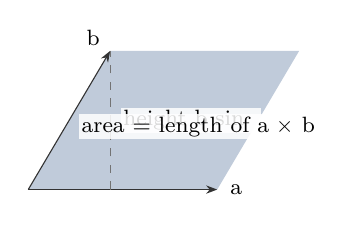
\begin{tikzpicture}[line join=round]
\fill[FAUblue!25] (0.752,-2.992) -- (3.152,-2.992) -- (4.192,-1.232) -- (1.792,-1.232) -- (0.752,-2.992) -- cycle;
\draw[-{Stealth[length=4pt]},black!80] (0.752,-2.992) -- (3.152,-2.992);
\draw[-{Stealth[length=4pt]},black!80] (0.752,-2.992) -- (1.792,-1.232);
\draw[black!55,dashed] (1.792,-2.992) -- (1.792,-1.232);
\node[anchor=west,fill=white,fill opacity=0.85,text opacity=1,inner sep=1pt,font=\footnotesize] at (3.278,-2.992) {a};
\node[anchor=east,fill=white,fill opacity=0.85,text opacity=1,inner sep=1pt,font=\footnotesize] at (1.702,-1.070) {b};
\node[anchor=west,fill=white,fill opacity=0.85,text opacity=1,inner sep=1pt,font=\footnotesize] at (1.918,-2.112) {height b sin α};
\node[fill=white,fill opacity=0.85,text opacity=1,inner sep=1pt,font=\footnotesize] at (2.912,-2.192) {area = length of a \ensuremath{\times} b};
\end{tikzpicture}\par\smallskip{\small\raggedright \textbf{Length of the cross product.} The parallelogram spanned by \textit{a} and \textit{b} has base |\textit{a}| and height |\textit{b}| sin \textit{α}, so its area is |\textit{a} \ensuremath{\times} \textit{b}|. The vector \textit{a} \ensuremath{\times} \textit{b} itself points out of the page.\par}\end{minipage}
\end{center}

\begin{workedbox}{Example \ensuremath{\cdot} a cross product}
\Needspace{5\baselineskip}
\begin{enumerate}
\item \textit{a} = (1, 2, 0)\textsuperscript{T}, \textit{b} = (0, 1, 3)\textsuperscript{T}.
\item \textit{a} \ensuremath{\times} \textit{b} = (2 \ensuremath{\cdot} 3 \ensuremath{-} 0 \ensuremath{\cdot} 1, 0 \ensuremath{\cdot} 0 \ensuremath{-} 1 \ensuremath{\cdot} 3, 1 \ensuremath{\cdot} 1 \ensuremath{-} 2 \ensuremath{\cdot} 0)\textsuperscript{T} = (6, \ensuremath{-}3, 1)\textsuperscript{T}.
\item Its length is \ensuremath{\sqrt{36\, +\, 9\, +\, 1}} \ensuremath{\approx} 6.78, the area of the parallelogram spanned by \textit{a} and \textit{b}.
\end{enumerate}

Check perpendicularity: (6, \ensuremath{-}3, 1) \ensuremath{\cdot} (1, 2, 0) = 6 \ensuremath{-} 6 + 0 = 0 and (6, \ensuremath{-}3, 1) \ensuremath{\cdot} (0, 1, 3) = 0 \ensuremath{-} 3 + 3 = 0.
\end{workedbox}
\end{keepsection}

\begin{keepsection}
\Needspace{17\baselineskip}
\section{B.6 Angles in the plane: atan(x, y), not arctan of the ratio}

\Needspace{14\baselineskip}
Cartesian, cylindrical and spherical coordinates, their unit vectors and their path, area and volume elements are collected in Appendix A. One point from the notes deserves its own card, because it causes most sign errors: the polar angle of a point needs both coordinates, not just their ratio.

\begin{equationcard}{The two-argument angle}
\[ \begin{gathered} {φ}\, =\, \text{atan}({x},\, {y}) \\ \text{atan}({x},\, {y})\, =\, \arctan \left(\dfrac{{y}}{{x}}\right)\, \text{for}\, {x}\, >\, 0,\, \arctan \left(\dfrac{{y}}{{x}}\right)\, \pm \, π\, \text{for}\, {x}\, <\, 0,\, \pm \dfrac{π}{2}\, \text{for}\, {x}\, =\, 0 \end{gathered} \]
{\small \emph{Read it as: “phi is the angle of the point (x, y), worked out from both coordinates”.}\par For \textit{x} \ensuremath{<} 0 add π when \textit{y} \ensuremath{\geq} 0 and subtract π when \textit{y} \ensuremath{<} 0; for \textit{x} = 0 take +{\small\ensuremath{\dfrac{π}{2}}} or \ensuremath{-}{\small\ensuremath{\dfrac{π}{2}}} by the sign of \textit{y}; at the origin the angle is undefined. This gives \ensuremath{-}π \ensuremath{<} \textit{φ} \ensuremath{\leq} π; for the range [0, 2π) add 2π to negative values. arctan({\small\ensuremath{\dfrac{{y}}{{x}}}}) alone only covers quadrants I and IV.}
\end{equationcard}

Example: the point (\ensuremath{-}1, \ensuremath{-}1) has {\small\ensuremath{\dfrac{{y}}{{x}}}} = 1, so arctan gives {\small\ensuremath{\dfrac{π}{4}}}, which points into quadrant I. atan(\ensuremath{-}1, \ensuremath{-}1) = {\small\ensuremath{\dfrac{π}{4}}} \ensuremath{-} π = \ensuremath{-}{\small\ensuremath{\dfrac{3π}{4}}}, or {\small\ensuremath{\dfrac{5π}{4}}} in [0, 2π). The same rule gives the phase of a complex number (B.8). The notes write the arguments in the order atan(\textit{x}, \textit{y}); a calculator's or a program's atan2 usually takes (\textit{y}, \textit{x}), so check the order before you trust a result.
\end{keepsection}

\begin{keepsection}
\Needspace{16\baselineskip}
\section{B.7 Systems of linear equations}

\Needspace{13\baselineskip}
Network analysis produces systems of linear equations: \textit{M} equations in \textit{N} unknowns, written as \textit{A} \textit{x} = \textit{b} with the coefficient matrix \textit{A}, the unknowns \textit{x} and the right-hand side \textit{b}. In circuit problems the method gives exactly as many independent equations as unknowns, so \textit{A} is square and \textbf{regular} and the system has exactly one solution.

\begin{equationcard}{When a square system has exactly one solution}
\[ \begin{gathered} {A}\, {x}\, =\, {b}\, \text{has}\, \text{one}\, \text{solution}\, \Leftrightarrow \, \text{det}\, {A}\, ≠\, 0\, \Leftrightarrow \, \text{rank}\, {A}\, =\, {N} \\ {x}\, =\, {A}^{-1}\, {b} \end{gathered} \]
{\small \emph{Read it as: “a square system has one solution exactly when the determinant of A is not zero”.}\par These statements are equivalent for a square \textit{A}: the system has exactly one solution, \textit{A} is invertible, det \textit{A} \ensuremath{\neq} 0, rank \textit{A} = \textit{N}. Swapping equations, multiplying one by a nonzero number and adding one to another never change the solutions.}
\end{equationcard}

\begin{equationcard}{Gaussian elimination}
\[ \begin{gathered} \text{forward}\, \text{elimination}\, \to \, \text{upper}\, \text{triangle}\, \to \, \text{back}\, \text{substitution} \end{gathered} \]
{\small Forward: use one equation to remove \textit{x}\textsubscript{1} from all the others, then repeat with \textit{x}\textsubscript{2} in what is left, until the last equation contains only \textit{x}\textsubscript{\textit{N}}. Back: solve for \textit{x}\textsubscript{\textit{N}}, then \textit{x}\textsubscript{\textit{N}\ensuremath{-}1}, and so on. It works for every system, including over- and underdetermined ones. To limit rounding errors, eliminate with the largest available coefficient (partial pivoting).}
\end{equationcard}

\begin{workedbox}{Example \ensuremath{\cdot} Gaussian elimination}
\Needspace{8\baselineskip}
\begin{enumerate}
\item Solve \textit{x}\textsubscript{1} + \textit{x}\textsubscript{2} + \textit{x}\textsubscript{3} = 6, 2\textit{x}\textsubscript{1} \ensuremath{-} \textit{x}\textsubscript{2} + \textit{x}\textsubscript{3} = 3, \textit{x}\textsubscript{1} + 2\textit{x}\textsubscript{2} \ensuremath{-} \textit{x}\textsubscript{3} = 2.
\item Subtract twice the first equation from the second and once from the third: \ensuremath{-}3\textit{x}\textsubscript{2} \ensuremath{-} \textit{x}\textsubscript{3} = \ensuremath{-}9 and \textit{x}\textsubscript{2} \ensuremath{-} 2\textit{x}\textsubscript{3} = \ensuremath{-}4.
\item Add a third of the new second equation to the new third: \ensuremath{-}{\small\ensuremath{\dfrac{7}{3}}} \textit{x}\textsubscript{3} = \ensuremath{-}7, so \textit{x}\textsubscript{3} = 3.
\item Back substitution: \ensuremath{-}3\textit{x}\textsubscript{2} \ensuremath{-} 3 = \ensuremath{-}9 gives \textit{x}\textsubscript{2} = 2, and \textit{x}\textsubscript{1} = 6 \ensuremath{-} 2 \ensuremath{-} 3 = 1.
\end{enumerate}

Check in the original third equation: 1 + 4 \ensuremath{-} 3 = 2.
\end{workedbox}

\begin{equationcard}{Cramer's rule}
\[ \begin{gathered} {x}_{{j}}\, =\, \dfrac{\text{det}\, {A}_{{j}}}{\text{det}\, {A}} \end{gathered} \]
{\small \emph{Read it as: “x j is the determinant of A with column j replaced by b, over the determinant of A”.}\par \textit{A}\textsubscript{\textit{j}} is \textit{A} with its \textit{j}-th column replaced by \textit{b}. Only for regular square systems, and expensive for many unknowns, because every unknown needs a determinant of its own.}
\end{equationcard}

\begin{workedbox}{Example \ensuremath{\cdot} Cramer's rule}
\Needspace{5\baselineskip}
\begin{enumerate}
\item Solve 3\textit{x}\textsubscript{1} + 2\textit{x}\textsubscript{2} = 7, \textit{x}\textsubscript{1} \ensuremath{-} \textit{x}\textsubscript{2} = \ensuremath{-}1. det \textit{A} = 3 \ensuremath{\cdot} (\ensuremath{-}1) \ensuremath{-} 2 \ensuremath{\cdot} 1 = \ensuremath{-}5 \ensuremath{\neq} 0.
\item Replace the first column by \textit{b}: det \textit{A}\textsubscript{1} = 7 \ensuremath{\cdot} (\ensuremath{-}1) \ensuremath{-} 2 \ensuremath{\cdot} (\ensuremath{-}1) = \ensuremath{-}5, so \textit{x}\textsubscript{1} = 1.
\item Replace the second column: det \textit{A}\textsubscript{2} = 3 \ensuremath{\cdot} (\ensuremath{-}1) \ensuremath{-} 7 \ensuremath{\cdot} 1 = \ensuremath{-}10, so \textit{x}\textsubscript{2} = 2.
\end{enumerate}

Check: 3 + 4 = 7 and 1 \ensuremath{-} 2 = \ensuremath{-}1.
\end{workedbox}

\begin{equationcard}{Too many or too few equations}
\[ \begin{gathered} {x}_{\text{opt}}\, =\, ({A}^{\mathrm{T}}{A})^{-1}\, {A}^{\mathrm{T}}\, {b} \end{gathered} \]
{\small \textbf{Overdetermined} (\textit{M} \ensuremath{>} \textit{N} equations, rank \textit{N}): the equations usually contradict each other, and the best compromise \textit{x}\textsubscript{opt} minimises the sum of the squared errors. Note: the notes print (\textit{A} \textit{A}\textsuperscript{T})\textsuperscript{\ensuremath{-}1}; for an \textit{M} \ensuremath{\times} \textit{N} matrix with \textit{M} \ensuremath{>} \textit{N} that product is \textit{M} \ensuremath{\times} \textit{M} and never invertible, so the least-squares formula must use \textit{A}\textsuperscript{T}\textit{A}, which is \textit{N} \ensuremath{\times} \textit{N} and invertible exactly when rank \textit{A} = \textit{N}. \textbf{Underdetermined} (rank \textit{A} \ensuremath{<} \textit{N}): if any solution exists (rank [\textit{A} | \textit{b}] = rank \textit{A}), the solutions form a family with \textit{N} \ensuremath{-} rank \textit{A} free parameters.}
\end{equationcard}
\end{keepsection}

\begin{keepsection}
\Needspace{16\baselineskip}
\section{B.8 Complex numbers in the course's notation}

\Needspace{13\baselineskip}
Alternating-current analysis (Chapter 6) runs on complex numbers. Electrical engineering writes the imaginary unit as j, because \textit{i} already means a current, and marks a complex quantity with an underline, \underline{\textit{x}}. The full treatment is in the MEI Chapter 4 guide; this section collects the rules in the EEI notation.

\begin{equationcard}{Cartesian and exponential form}
\[ \begin{gathered} \underline{{x}}\, =\, {x}_{\text{Re}}\, +\, \mathrm{j}\, {x}_{\text{Im}},\, \mathrm{j}^{2}\, =\, -1 \\ \underline{{x}}\, =\, |\underline{{x}}|\, \mathrm{e}^{\mathrm{j}{φ}}\, =\, |\underline{{x}}|(\cos \, {φ}\, +\, \mathrm{j}\, \sin \, {φ}) \end{gathered} \]
{\small \emph{Read it as: “x is its real part plus j times its imaginary part, or its magnitude times e to the j phi”.}\par \textit{x}\textsubscript{Re} = Re\{\underline{\textit{x}}\} and \textit{x}\textsubscript{Im} = Im\{\underline{\textit{x}}\} are real. The magnitude is |\underline{\textit{x}}| = \ensuremath{\sqrt{{x}_{\text{Re}}^{2}\, +\, {x}_{\text{Im}}^{2}}} (the notes put a hat over the letter) and the phase is \textit{φ} = atan(\textit{x}\textsubscript{Re}, \textit{x}\textsubscript{Im}) from B.6, not arctan of the ratio. The second line is Euler's formula.}
\end{equationcard}

\begin{equationcard}{Conjugate}
\[ \begin{gathered} \underline{{x}}^{*}\, =\, {x}_{\text{Re}}\, -\, \mathrm{j}\, {x}_{\text{Im}}\, =\, |\underline{{x}}|\, \mathrm{e}^{-\mathrm{j}{φ}} \\ \underline{{x}}\, \underline{{x}}^{*}\, =\, |\underline{{x}}|^{2} \\ \text{Re}\{\underline{{x}}\}\, =\, \dfrac{1}{2}(\underline{{x}}\, +\, \underline{{x}}^{*}) \\ \text{Im}\{\underline{{x}}\}\, =\, \dfrac{1}{2\mathrm{j}}(\underline{{x}}\, -\, \underline{{x}}^{*}) \end{gathered} \]
{\small The asterisk reflects the point in the real axis: same magnitude, opposite phase.}
\end{equationcard}

\begin{equationcard}{Arithmetic}
\[ \begin{gathered} \underline{{x}}_{1}\, \pm \, \underline{{x}}_{2}\, =\, ({x}_{\text{Re}1}\, \pm \, {x}_{\text{Re}2})\, +\, \mathrm{j}({x}_{\text{Im}1}\, \pm \, {x}_{\text{Im}2}) \\ \underline{{x}}_{1}\, \underline{{x}}_{2}\, =\, |\underline{{x}}_{1}|\, |\underline{{x}}_{2}|\, \mathrm{e}^{\mathrm{j}(φ_{1}\, +\, φ_{2})} \\ \dfrac{\underline{{x}}_{1}}{\underline{{x}}_{2}}\, =\, \dfrac{|\underline{{x}}_{1}|}{|\underline{{x}}_{2}|}\, \mathrm{e}^{\mathrm{j}(φ_{1}\, -\, φ_{2})} \end{gathered} \]
{\small Add in Cartesian form, like vectors. Multiply and divide in exponential form: magnitudes multiply or divide, phases add or subtract. In Cartesian form a quotient is expanded with the conjugate of the denominator.}
\end{equationcard}

\begin{equationcard}{Multiplying by j}
\[ \begin{gathered} \mathrm{j}\, \underline{{x}}\, =\, \mathrm{e}^{\mathrm{j}π/2}\, \underline{{x}}\, =\, -{x}_{\text{Im}}\, +\, \mathrm{j}\, {x}_{\text{Re}} \\ \dfrac{\underline{{x}}}{\mathrm{j}}\, =\, -\mathrm{j}\, \underline{{x}}\, =\, {x}_{\text{Im}}\, -\, \mathrm{j}\, {x}_{\text{Re}} \end{gathered} \]
{\small Multiplying by j turns a phasor a quarter turn counterclockwise (+{\small\ensuremath{\dfrac{π}{2}}}); dividing by j turns it a quarter turn clockwise (\ensuremath{-}{\small\ensuremath{\dfrac{π}{2}}}). This is the source of the \ensuremath{\pm}90° phase shifts of ideal coils and capacitors.}
\end{equationcard}

\begin{equationcard}{Powers and roots}
\[ \begin{gathered} \underline{{x}}^{{N}}\, =\, |\underline{{x}}|^{{N}}\, \mathrm{e}^{\mathrm{j}{φ}{N}} \\ {w}_{{n}}\, =\, |\underline{{x}}|^{1/{N}}\, \mathrm{e}^{\mathrm{j}(φ\, +\, 2π{n})/{N}},\, {n}\, =\, 0,\, 1,\, …,\, {N}\, -\, 1 \end{gathered} \]
{\small An \textit{N}-th root has \textit{N} different values, spread evenly round a circle. In particular \textit{x}\textsuperscript{\textit{N}} = 1 is solved by e\textsuperscript{j2π\textit{n}/\textit{N}}.}
\end{equationcard}

\Needspace{14\baselineskip}
\begin{center}
\begin{minipage}[t]{0.950\linewidth}\centering
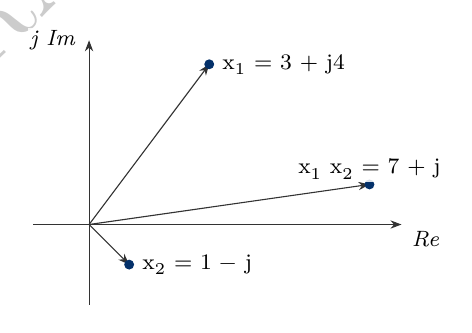
\begin{tikzpicture}[line join=round]
\draw[-{Stealth[length=4pt]},black!80] (0.432,-2.772) -- (5.112,-2.772);
\node[anchor=west,fill=white,fill opacity=0.85,text opacity=1,inner sep=1pt,font=\footnotesize] at (5.202,-2.952) {\textit{Re}};
\draw[-{Stealth[length=4pt]},black!80] (1.144,-3.789) -- (1.144,-0.432);
\node[anchor=east,fill=white,fill opacity=0.85,text opacity=1,inner sep=1pt,font=\footnotesize] at (1.018,-0.432) {\textit{j Im}};
\draw[-{Stealth[length=4pt]},black!80] (1.144,-2.772) -- (2.670,-0.737);
\draw[-{Stealth[length=4pt]},black!80] (1.144,-2.772) -- (1.653,-3.281);
\draw[-{Stealth[length=4pt]},black!80] (1.144,-2.772) -- (4.705,-2.263);
\fill[FAUblue] (2.670,-0.737) circle (0.063);
\fill[FAUblue] (1.653,-3.281) circle (0.063);
\node[anchor=west,fill=white,fill opacity=0.85,text opacity=1,inner sep=1pt,font=\footnotesize] at (2.796,-0.737) {x\textsubscript{1} = 3 + j4};
\node[anchor=west,fill=white,fill opacity=0.85,text opacity=1,inner sep=1pt,font=\footnotesize] at (1.779,-3.281) {x\textsubscript{2} = 1 \ensuremath{-} j};
\fill[FAUblue] (4.705,-2.263) circle (0.063);
\node[fill=white,fill opacity=0.85,text opacity=1,inner sep=1pt,font=\footnotesize] at (4.705,-2.065) {x\textsubscript{1} x\textsubscript{2} = 7 + j};
\end{tikzpicture}\par\smallskip{\small\raggedright \textbf{A product in the complex plane.} \underline{\textit{x}}\textsubscript{1} = 3 + j4 and \underline{\textit{x}}\textsubscript{2} = 1 \ensuremath{-} j. Their product 7 + j has magnitude 5 \ensuremath{\cdot} \ensuremath{\sqrt{2}} and phase 53.1° \ensuremath{-} 45°.\par}\end{minipage}
\end{center}

\begin{workedbox}{Example \ensuremath{\cdot} multiply, divide, take roots}
\Needspace{7\baselineskip}
\begin{enumerate}
\item \underline{\textit{x}}\textsubscript{1} = 3 + j4, \underline{\textit{x}}\textsubscript{2} = 1 \ensuremath{-} j. Product: (3 + j4)(1 \ensuremath{-} j) = 3 \ensuremath{-} j3 + j4 \ensuremath{-} j\textsuperscript{2}4 = 7 + j.
\item Quotient: multiply top and bottom by 1 + j: {\small\ensuremath{\dfrac{(3\, +\, \mathrm{j}4)(1\, +\, \mathrm{j})}{2}}} = {\small\ensuremath{\dfrac{-1\, +\, \mathrm{j}7}{2}}} = \ensuremath{-}0.5 + j3.5.
\item Phase of \underline{\textit{x}}\textsubscript{1}: atan(3, 4) = arctan {\small\ensuremath{\dfrac{4}{3}}} \ensuremath{\approx} 0.927 rad \ensuremath{\approx} 53.1° (quadrant I), magnitude 5.
\item Cube roots of 8j = 8e\textsuperscript{jπ/2}: magnitude 2, phases {\small\ensuremath{\dfrac{π}{6}}}, {\small\ensuremath{\dfrac{5π}{6}}}, {\small\ensuremath{\dfrac{3π}{2}}}, giving \ensuremath{\sqrt{3}} + j, \ensuremath{-}\ensuremath{\sqrt{3}} + j and \ensuremath{-}2j.
\end{enumerate}

Check: |7 + j| = \ensuremath{\sqrt{50}} = 5\ensuremath{\sqrt{2}} = |\underline{\textit{x}}\textsubscript{1}| |\underline{\textit{x}}\textsubscript{2}|, and (\ensuremath{-}2j)\textsuperscript{3} = \ensuremath{-}8j\textsuperscript{3} = 8j.
\end{workedbox}
\end{keepsection}


\vfill{\small Personal reference sheet based on the Electrical Engineering 1 lecture notes, Chapter 7 “Mathematical Appendix” (printed pages 531–597), rearranged and explained in my own words, mostly with my own examples (the B.1 semicircle is the notes’ example, worked in my own words); the original figures and tables are not reproduced. Not an official FAU publication; check details against the current course material. Made by \textbf{Thanate Amornjiraporn (Focus)}.}

\end{document}
